\documentclass[a4paper,12pt]{article}

% Se vuoi che il pdf sia in formato mobile, decommenta la linea qui sotto e commenta la prima linea del codice
%\documentclass[1pt]{article}
\usepackage{enumitem}
\usepackage[paper size={90mm, 160mm},left=2mm,right=2mm,top=2mm,bottom=2mm,nohead]{geometry}
\usepackage{microtype}
\setlist[itemize]{leftmargin=*}


\usepackage{float}
\usepackage{url}
\usepackage{xcolor}
\usepackage{pdfpages}
\usepackage{graphicx}


%Comando per creare nuove definizioni stile blocco
\newcommand{\definition}[2]{
	\begin{table}[H]
	\centering
		\begin{tabular}{|p{0.9\linewidth}}
		\textbf{#1}\\ %Titolo della definzione
		#2\\%Testo della definizione
		\end{tabular}
	\end{table}
	\noindent
}

\newcommand{\df}[2]{\definition{#1}{#2}}

%%%%%%%%%%%%%%%%%%%%%%%%%%%%%%%%%%%%%%%%%%%%%%%%%%%%%%%%%%%%%%%%%%%%%
%      INSBOX --- macros for inserting pictures into paragraphs     %
%       Micha\l{} Gulczy\'nski, Szczecin, Jan 1996 / Feb 1998       %
%                     mgulcz@we.tuniv.szczecin.pl                   %
%%%%%%%%%%%%%%%%%%%%%%%%%%%%%%%%%%%%%%%%%%%%%%%%%%%%%%%%%%%%%%%%%%%%%
%
%  version 2.2
%
%  available macros:
%    * \InsertBoxC{anybox}
%        insert a centered box (use int _inside_ a paragraph)
%    * \InsertBoxL{after_line}{anybox}[correction]
%    * \InsertBoxR{after_line}{anybox}[correction]
%        insert a box in the left/right after specified number of lines;
%        correction specified in square brackets is optional;
%        both macros should be called _before_ a paragraph
%    * \MoveBelowBox
%        start a new paragraph just below the current frame
%
%  see the demo.tex file for more information
%

\catcode`\@ = 11
%
%  Margin between the text and the box:
\newdimen\@InsertBoxMargin
\@InsertBoxMargin = 2mm
%
%  definition of \ParShape, an inproved version of plain \parshape
%
\newcount\@numlines    % sum: m_1+...+m_n
\newcount\@linesleft   % counter used when reading lines of \ParShape
\def\ParShape{%
    \@numlines = 0
    \def\@parshapedata{ }% here we'll collect data for plain \parshape
    \afterassignment\@beginParShape
    \@linesleft
}%
\def\@beginParShape{%
    \ifnum \@linesleft = 0
      \let\@whatnext = \@endParShape
    \else
      \let\@whatnext = \@readnextline
    \fi
    \@whatnext
}%
\def\@endParShape{%
    \global\parshape = \@numlines \@parshapedata
}%
\def\@readnextline#1 #2 #3 {% #1 #2 #3 are: m_i, leftskip_i, rightskip_i
    \ifnum #1 > 0
      \bgroup  % I want to keep changes of \dimen0 and \count0 local
        \dimen0 = \hsize
        \advance \dimen0 by -#2  % \parshape requires left skip and
        \advance \dimen0 by -#3  % _length_of_line_ (not right skip!)
        \count0 = 0
        \loop
          \global\edef\@parshapedata{%
            \@parshapedata    % add to \@parshapedata:
            #2                % left skip
            \space            % a space
            \the\dimen0       % length of line
            \space            % another space
          }%
          \advance \count0 by 1
          \ifnum \count0 < #1
        \repeat
      \egroup
      \advance \@numlines by #1
    \fi
    \advance \@linesleft by -1
    \@beginParShape
}%
%
%  \InsertBoxC, \InsertBoxL, \InsertBoxR
%
\newbox\@boxcontent     % box containing the picture to be inserted
\newcount\@numnormal    % number of leading lines to typeset normally
\newdimen\@framewidth   % width of the frame
\newdimen\@wherebottom  % position of frame's bottom
\newif\if@byframe       % true if we are just beside the frame
\@byframefalse
%
%
\def\InsertBoxC#1{%
  \leavevmode
  \vadjust{
    \vskip \@InsertBoxMargin
    \hbox to \hsize{\hss#1\hss}
    \vskip \@InsertBoxMargin
  }%
}%
\def\InsertBoxL#1#2{%
  \@numnormal = #1
  \setbox\@boxcontent = \hbox{#2}%
  \let\@side = 0
  \futurelet \@optionalparameter \@InsertBox
}
\def\InsertBoxR#1#2{%
  \@numnormal = #1
  \setbox\@boxcontent = \hbox{#2}%
  \let\@side = 1
  \futurelet \@optionalparameter \@InsertBox
}%
\def\@InsertBox{%
  \ifx \@optionalparameter [
    \let\@whatnext = \@@InsertBoxCorrection
  \else
    \let\@whatnext = \@@InsertBoxNoCorrection
  \fi
  \@whatnext
}%
\def\@@InsertBoxCorrection[#1]{%
  \ifx \@side 0
    \@@InsertBox{#1}{0}{{\the\@framewidth} 0cm}%
  \else
    \@@InsertBox{#1}{1}{0cm {\the\@framewidth}}%
  \fi
}%
\def\@@InsertBoxNoCorrection{%
  \@@InsertBoxCorrection[0]%
}%
\def\@@InsertBox#1#2#3{%
  \MoveBelowBox
  \@byframetrue
  % \@wherebottom = \pagetotal + (\@numnormal * \baselineskip) +
  %                 (height of \@boxcontent) + (2 * \@InsertBoxMargin)
  \@wherebottom = \baselineskip
  \multiply \@wherebottom by \@numnormal
  \advance \@wherebottom by 2\@InsertBoxMargin
  \advance \@wherebottom by \ht\@boxcontent
  \advance \@wherebottom by \pagetotal
  % I have no idea why, but \InsertBox called at the top of a page
  % calculates space for the box one line too big
  \ifdim \pagetotal = 0cm
    \advance \@wherebottom by -\baselineskip  % ^ reduction
  \fi
  % add the correction
  \advance \@wherebottom by #1\baselineskip
  % \@framewidth = (width of \@boxcontent} + \@InsertboxMargin
  \@framewidth = \wd\@boxcontent
  \advance \@framewidth by \@InsertBoxMargin
  %
  \bgroup  % to keep changes of \dimen0 local
    % check if the box fits in the page
    \ifdim \pagetotal = 0cm
      \dimen0 = \vsize
    \else
      \dimen0 = \pagegoal
    \fi
    \ifdim \@wherebottom > \dimen0
      % print a warning message ...
      \immediate\write16{+--------------------------------------------------------------+}%
      \immediate\write16{| The box will not fit in the page. Please, re-edit your text. |}%
      \immediate\write16{+--------------------------------------------------------------+}%
      % ... and mark this place in document with a black box
      \vrule width \overfullrule
    \fi
  \egroup
  \prevgraf = 0
  % insert the box in the left (if #2 = 0) or in the right (if #2 = 1)
  \vbox to 0cm{%
    \dimen0 = \baselineskip
    \multiply \dimen0 by \@numnormal
    \advance \dimen0 by -\baselineskip
    \setbox0 = \hbox{y}%
    \vskip \dp0
    \vskip \dimen0
    \vskip \@InsertBoxMargin
    \ifnum #2 = 1
      \vtop{\noindent \hbox to \hsize{\hss \box\@boxcontent}}%
    \else
      \vtop{\noindent \box\@boxcontent}%
    \fi
    \vss
  }%
  % I have no idea why, but this is really necessary
  \vglue -\parskip
  \vskip -\baselineskip
  % each following paragraph needs to be formatted properly
  \everypar = {%
    % are we already below the bottom of the box?
    \ifdim \pagetotal < \@wherebottom
      % no...
      \bgroup  % to keep some changes local
        % let's calculate parameters for \ParShape
        \dimen0 = \@wherebottom
        \advance \dimen0 by -\pagetotal
        \divide \dimen0 by \baselineskip
        \count1 = \dimen0
        \advance \count1 by 1
        \advance \count1 by -\@numnormal
        \ifnum #2 = 1
          \ParShape = 3
                      {\the\@numnormal}   0cm   0cm
                      {\the\count1}       0cm   {\the\@framewidth}
                      1                   0cm   0cm
        \else
          \ParShape = 3
                      {\the\@numnormal}   0cm                  0cm
                      {\the\count1}       {\the\@framewidth}   0cm
                      1                   0cm                  0cm
        \fi
      \egroup
    \else
      % yes!
      \@restore@    % it's time to end everything
    \fi
  }%
  % this definition isn't very necessary --- just in case the paragraph
  % following \InsertBoxL or \InsertBoxR has fewer lines that the
  % first argument of the macro
  \def\par{%
      \endgraf
      \global\advance \@numnormal by -\prevgraf
      \ifnum \@numnormal < 0
        \global\@numnormal = 0
      \fi
      \prevgraf = 0
  }%
}%
%
%  call this macro to move the current position just below the
%  current frame
%
\def\MoveBelowBox{%
  \par
  \if@byframe
    \global\advance \@wherebottom by -\pagetotal
    \ifdim \@wherebottom > 0cm
      \vskip \@wherebottom
    \fi
    \@restore@
  \fi
}%
%
%  normal settings are as follows:
%
\def\@restore@{%
    \global\@wherebottom = 0cm
    \global\@byframefalse
    \global\everypar = {}%
    \global\let \par = \endgraf
    \global\parshape = 1 0cm \hsize
}%
%
%  someone told me that in LaTeX there is no \pageno counter;
%  the counterpart is \c@page
%
\ifx \documentclass \@Dont@Know@What@It@Is@
\else
  \let \pageno = \c@page
\fi


\catcode`\@ = 12

\newcommand{\lessonDate}[1]{\InsertBoxR{0}{\tiny{#1}}}

\newcommand{\E}{\`E\space}

\usepackage{listings}
\lstset{language=C++,
                keywordstyle=\color{blue},
                stringstyle=\color{red},
                commentstyle=\color{green},
                morecomment=[l][\color{magenta}]{\#}
}

\begin{document}

\begin{titlepage}
\begin{center}
	\Large{\textbf{Gestione dell'informazione Geospaziale}}
\vfill
\normalsize{Caccaro Sebastiano}\\
\normalsize{A.A.2019/2020}
\end{center}
\end{titlepage}
\tableofcontents

\clearpage


%Lunedi 7 ottobre
\lessonDate{7 Ottobre 2019}
\section{Introduzione}
\textbf{Geospaziale} tratta di dati sulla superficie terrestre. Posso trattare vari tipi di spazi, anche su unità di misura diverse, come lo spazio-tempo.

\subsection{Aspetti organizzativi}
\subsubsection{Obiettivi}
Concetti base:
\begin{itemize}
	\item Acquisizione dei dati
	\item Gestione dei dati: li mantengo in dei DBMS spaziali.
	\item Analisi dei dati, clustering (= raggruppare oggetti in base a criteri di omogeneità) ecc.
\end{itemize}

\subsubsection{Organizzazione del corso}
Il corso verrà così articolato:
\begin{itemize}
	\item Concetti base
	\item DBMS Spaziali
	\item Rappresentazione di oggetti in movimento
	\item Analisi dei dati spaziali.	
\end{itemize}

\textbf{Bisogna sapere PostgreSQL!}\\
L'esame consiste in un progetto più di un orale (potrebbe diventare una prova scritta all'ultima lezione del corso).\\
Il sito del corso è \url{homes.di.unimi.mdamiani/corsi/gig/}\\
\textbf{User}: gis7 \textbf{Pwd:} sql07sql

\subsubsection{Materiale}
\E presente un libro in formato PDF sul sito della docente.


\subsection{Concetti Base}
\subsubsection{Esempio di OpenStreetMaps}
OpenStreetMaps è una \textbf{mappa} aperta \textbf{collaborativa}, sostanzialmente un disegno. Ma non ci interessano i colori delle strade ecc. Cosa vuol dire Mappa Collaborativa?
\begin{itemize}
 \item \textbf{Mappa} è una banca dati che contiene informazioni geografiche coerenti, che poi vengono rappresentate tramite una mappa.
 \item \textbf{Collaborativa} la base di dati è modificabile da chiunque.\\
\end{itemize}


Costruire mappe è sempre stato altamente dispendioso, sopratutto per quanto riguarda l'acquisizione dei dati. OpenStreetMaps rende facile il reperimento e l'uso di dati spaziali.

\subsubsection{Spazio}
Parliamo di spazio geometrico con longitudine e latitudine, che vogliono una posizione e un sistema di riferimento. \E però molto più facile usare lo spazio cartesiano. Lo spazio simbolico invece rappresenta dei luoghi anche in base alla loro funzione (esempio cartine indoor). A seconda del tipo di spazio che sto analizzando, cambia anche la nozione di distanza. Ad esempio, come misuro la distanza in ambiente indoor?\\
Un oggetto può avere vari tipi di proprietà:
\begin{itemize}
\item \textbf{Geometriche}: forma
\item \textbf{Topografiche}: i collegamenti, a mo di grafo
\item \textbf{Tematiche}: caratteristiche, ad esempio i il numero di abitanti di un edificio
\end{itemize}

Ci possono essere movimenti di tipo:
\begin{itemize}
\item \textbf{Continuo:} ad esempio, movimento di palla nello spazio.
\item \textbf{Discreto:} ho un numero di posizioni finito, ad esempio posso essere in un dato momento solo sotto una cella telefonica.
\end{itemize}

%Possibile spostare a mappe
\E importantissimo poter visualizzare i dati. Altrimenti, non riesco a farmi un'idea di cosa ho in mano.

\subsubsection{Acquisizione dei dati}
Ci sono vari strumenti e metodi (arei, GPS, ecc.).\\
La posizione non è mai precisa al 100\%. I dati geospaziali dovrebbero essere sempre accompagnati anche dalla misura della loro incertezza.

\subsubsection{Trattamento dei dati}
Sono presenti varie tecnologie che permettono di gestire e trattare i dati raccolti:
\begin{itemize}
\item \textbf{Sistemi GIS}: piattaforme software (= programmoni) che mi permettono di:
	\begin{itemize}
		\item Acquisire dati: digitalizzarli, controllarne la correttezza, integrare dati eterogenei (con fonti e caratteristiche diverse).
		\item Archiviare e accedere ai dati
		\item Trattare i dati
		\item Visualizzare dati
	\end{itemize}
\item \textbf{DBMS spaziali}: DBMS normali arricchiti con tipi e operazioni per dati spaziali. Praticamente sono SQL con estensioni spaziali.
	
\item Package specializzati.
\end{itemize}

\lessonDate{11 Ottobre 2019}
\section{Coordinate Geospaziali}
\definition{Geodesia}{Disciplina che studia la forma della Terra, le sue dimensioni, i metodi per determinare la posizione dei punti sulla sua superficie.}

\definition{Cartografia}{Disciplina che ha per oggetto la rappresentazione grafica, in proporzioni ridotte, della superficie terrestre o di una parte di essa, dei suoi aspetti caratteristici, fenomeni che si svolgono e la preparazione e la costruzione delle carte geografiche.}

Le coordinate sono delle tuple di numerici che hanno senso in un sistema di riferimento (CRS - Coordinate Reference System). Bisogna distinguere due tipi di coordinate:
\begin{itemize}
\item \textbf{Coordinate Geografiche:} ex Latitudine e longitudine.
\item \textbf{Coordinate Proiettate:} ovvero proiettate su un piano.
\end{itemize}
\E possibile anche fornire delle coordinate indirette, come un indirizzo postale, IP, ecc. Questi metodi vengono poi mappati a coordinate.

\subsection{Coordinate Geografiche}
\definition{Meridiano}{Semicirconferenza che unisce i due poli.}
\definition{Meridiano di Greenwich}{Anche detto Meridiano Fondamentale". Meridiano di riferimento per il calcolo della circonferenza.}
\definition{Piano Equatoriale}{Piano che ha come proiezione l'equatore.}

\begin{figure}[H]
	\centering
	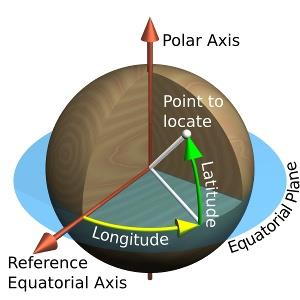
\includegraphics[width=.4\linewidth]{Immagini/LatLong.png}
\end{figure}

\subsection{Latitudine e longitudine}
\df{Longitudine}{Angolo sul piano di meridiano fra l'equatore e la linea passante per P e perpendicolare alla superficie terrestre. Indicata con phi.}\\
\df{Latitudine}{Angolo sul piano equatoriale formato dal piano del meridiano passante per P e il piano del meridiano fondamentale. Indicata con lambda}\\

Sia latitudine e longitudine sono angoli, quindi si misurano in gradi. Ma ci sono 2 modi per esprimerli:
\begin{itemize}
\item \textbf{Sistemi sessasegimali:} Misuro in sessantesimi.
\item \textbf{Sistemi digitali:} Misure in frazioni decimali di grado.
\end{itemize}

La longitudine è espressa fra \textbf{180 OVEST} e \textbf{180 EST} (-180 e 180). La latitudine è espresso fra \textbf{90 NORD} E \textbf{90 SUD} (0 -90 e 90). Per ovvi motivi, nei poli la longitudine non è definita.\\

\subsection{Distanza}
Chiaramente, per calcolare la distanza, non basta tirare una linea. La distanza più breve fra due punti, non è una linea retta sul piano.

\definition{Cerchio Massimo}{Circonferenza che risulta dall'intersezione di un piano passante per il centro e la superficie terrestre. Il cerchio massimo è un esempio di geodetica}
\definition{Distanza di Cerchio Massimo}{Distanza più breve tra 2 punti A e B è data dall'arco di cerchio massimo passante per A e B (con estremi A e B). Ipotesi di Terra sferica (errore stimato 0.3\%)}

\begin{figure}[H]
	\centering
	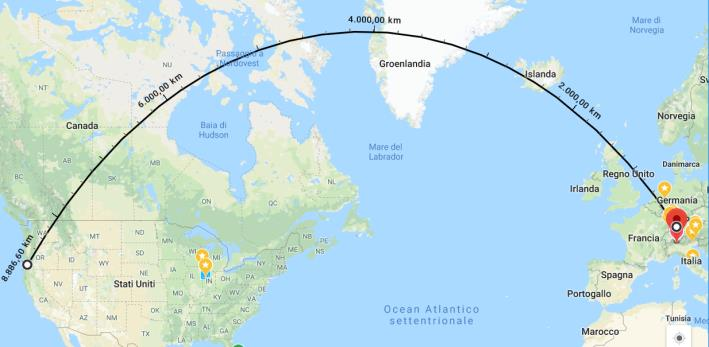
\includegraphics[width=.75\linewidth]{Immagini/CMax.png}
	\caption{Distanza più breve (di cerchio massimo) fra due punti sulla terra}
\end{figure}

\subsection{Forma della Terra}
La terrà non è una sfera, ci sono valli, montagne, ecc. Dobbiamo quindi stabilire una superficie di riferimento, un modello geometrico, \textbf{datum geodetico}. Una prima approssimazione potrebbe essere il geoide, che "taglia" le montagne e pone il livello di riferimento alla superficie del mare.
Sarebbe però troppo difficile da computare, quindi usiamo un modello regolare detto \textbf{Ellissoide}. Sono stati definiti vari tipi di ellissoide. Ciò è causato da vari fattori. Alcuni ellissoidi approssimano meglio alcune aree geografiche (es Europa, Italia ecc) (datum locale), mentre altri cercano di approssimare tutta la superficie terrestre senza fare troppe preferenze. La tendenza è quella di migrare verso dei modelli globali (datum globale), come WGS84, usato nel GPS.\\
Va da sè che latitudine e longitudine non sono sufficienti per identificare univocamente un punto, ma è necessario anche  il codice dell'ellissoide.

\begin{figure}[H]
	\centering
	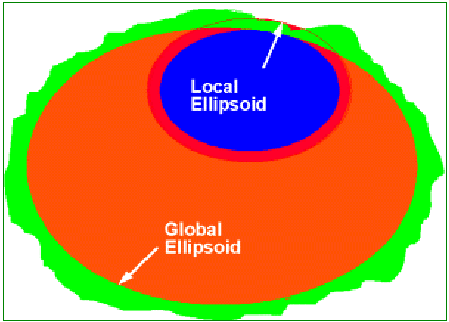
\includegraphics[width=.75\linewidth]{Immagini/Elix.png}
	\caption{Ellissoidi locali e globali}
\end{figure}

\subsubsection{Trasformazione di datum}
Può dover essere necessario eseguire delle trasformazioni di datum fra modelli geodetici differenti.

\subsection{Coordinate Proiettate}
Consistono sostanzialmente in un mapping da coordinate geografiche a coordinate cartesiane. \E possibile passare da una proiezione all'altra senza perdita di dettagli tramite alcune formulette matematiche.\\
Ovviamente, questa mappatura causa delle deformazioni, e in base a queste posso classificare le proiezioni:
\begin{itemize}
\item \textbf{Equivalenti:} mantengono le aree
\item \textbf{Conformi:} mantengono gli angoli
\item \textbf{Equidistanti: } mantengono le distanze
\end{itemize}
Non esistono proiezioni migliori, ma solo più ideali rispetto al contesto.
Generalmente ci viene \textbf{più facile} usare coordinate proiettate.
\lessonDate{14 Ottobre 2019}


\subsubsection{LatLong projection}
Latitudine e longitudine vengono usati come X e Y. Si utilizza perchè è molto semplice, senza troppi fronzoli. Si può usare quando non si hanno troppe esigenze di precisione.\\

\begin{figure}[H]
	\centering
	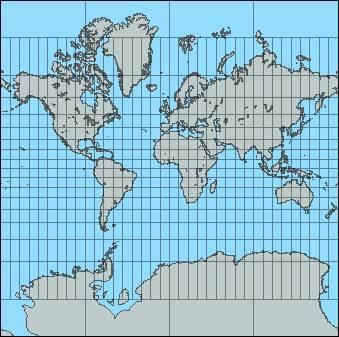
\includegraphics[width=.6\linewidth]{Immagini/LatLongProj}
	\caption{Proiezione LatLong}
\end{figure}

\subsubsection{Proiezione di Gauss}
Sta alla base di molte proiezioni, chiamata anche \textbf{Transverse Mercator}. \E una \textbf{proiezione conforme}, quindi preserva gli angoli. Introduce grosse deformazioni, per cui usa per aree non più grandi di 6 gradi di longitudine dall'equatore (circa 600km).\\
La proiezione di Guass è alla base di alcune proiezioni, fra cui:
\begin{itemize}
\item \textbf{UTM}: (Universal Trasverse Mercator). La terra è divisa in zone delimitate da 60 meridiani e da spicchi di 6 gradi di longitudine. le coordinate sono espresse in metri (x dal meridiano centrale, y dall'equatore). Per non avere coordinate negative, lo zero corrisponde a 500km.
\item \textbf{Proiezioni di Gauss-Boaga}: usata in Italia, e pensata da un italiano per il territorio italiano. Si divide la longitudine in due fusi (verticali). Anche in questo caso sono presenti delle false origini per avere sempre coordinate positive.
\end{itemize}

\begin{figure}[H]
	\centering
	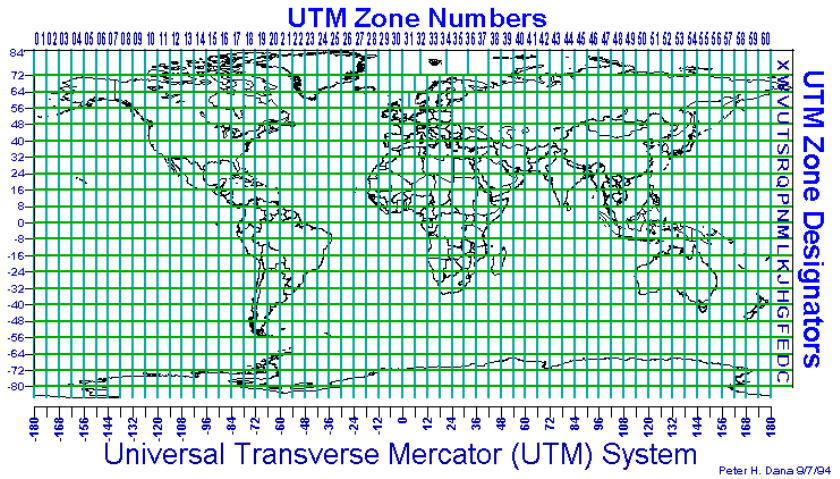
\includegraphics[width=\linewidth]{Immagini/UTM}
	\caption{Divisione in zone UTM}
\end{figure}

\begin{figure}[H]
	\centering
	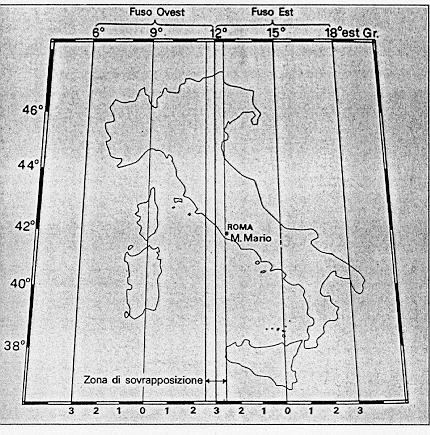
\includegraphics[width=0.6\linewidth]{Immagini/GaussBoaga}
	\caption{Proiezione di Gauss Boaga}
\end{figure}

\subsection{Sistema di coordinate Geografiche (CRS)}
Per stabilire un sistema di coordinate geografiche, ho bisogno di:
\begin{itemize}
\item Una proiezione cartografica
\item Una Datum geodetico
\end{itemize}

Le varie combinazioni di CRS sono delle stringhe definite da un gruppo chiamato \textbf{EPSG}, che identificano le varie coppie, come \texttt{EPSG 4326} ecc.

\subsubsection{Trasformazione dei sistemi di coordinate}
La trasformazione fra coordinate è lossless, perchè posso ricondurre ogni coordinata alle coordinate geografiche e viceversa. \E già più complicato passare fra due dati geoedici diversi.

\subsection{Scala}
Il concetto di scala è abbastanza banale. Nella cartografia tradizionale, il concetto di scala indica implicitamente anche la precisione di un dato, perchè non posso rappresentare oggetti più piccoli di un tot. Questo concetto è trasportato anche nella cartografica digitale, dove la scala può stare a indicare la cartografia di un dataset.\\
Più una scale è grande, più il rapporto è maggiore, e viceversa.

\lessonDate{18 Ottobre}
\section{Modelli dei dati e gestione dei dati spaziali}
Ho bisogno di formulare delle astrazione per poter visualizzare i dati in R\^2. Posso farlo in due modi:
\begin{itemize}
\item \textbf{Visione concettuale:} Realizzo delle astrazioni per visualizzare delle entità
\item \textbf{Visione basata su entità:} ho uno spazio in cui riesco a definire degli oggetti con forme geometriche e.g. curve di livello in un campo scalare o un campo vettoriale.
\end{itemize}

In R\^2 posso rappresentare:
\begin{itemize}
\item \textbf{Entità spaziali:} oggetti tra loro distinguibili e univocamente identificabili aventi una forma geometrica (e.g. vetta della montagna) 
\item \textbf{Campi:} funzione \texttt{f} che associa ad ogni punto di una regione \texttt{W} in \texttt{R\^2} un valore, che può essere:
	\begin{itemize}
	\item \texttt{Numerico:} campo scalare e.g. temperatura \texttt{f: W -> R}
	\item \texttt{Vettoriale}: campo vettoriale e.g. velocità \texttt{f:W -> R\^n}
	\end{itemize}
\end{itemize}

Ad esempio, potrei rappresentare una foresta come un campo (vettoriale o numerico) o come un poligono, cioè un'entità.

\subsection{Modelli per la rappresentazione dei dati spaziali}
Esistono vari modelli per rappresentare dati spaziali.
\subsubsection{Modello Vettoriale}
Utilizzato per la rappresentazione di entità spaziali. Rappresentata da un elemento geometrico (punto, linea, poligono). I tipi geometrici fondamentali sono in numero limitato, ad esempio le spline non sono importanti e non sempre definiti. Non mi serve avere poligoni molto complessi, dato che i sistemi GIS hanno una maggiore tolleranza (es un cerchio posso semplificarlo con un poligono a n lati).


\subsubsection{Modelli basato su tassellazione}
Utilizzato per la rappresentazione di campi. Il campo devo discretizzarlo, la funzione campo f è definita su uno spazio W discretizzato. La regione W è partizionata in forma regolare o non regolare e ad ogni regione associo un valore (è praticamente una mesh). Il modello più comune è quello raster.

\subsection{Raster}

La regione dello spazio è divisa con una matrice (regolare) e il sistema di coordinate definisce la posizione delle celle nello spazio. Ogni cella ha associato il valore (valore del campo in quella posizione). Può essere osservato subito o tramite interpolazione e può essere null. Posso avere più layers di raster sovrapposti per codificare più informazioni.\\
Ad esempio, ogni cella rappresenta una porzione di territorio. Posso avere layer sovrapposti: uno per la vegetazione, uno per la strada, una per l'altitudine, edifici, pressione etc.\\
Una differenza sostanziale delle immagini raster, oltre che ad avere n layer, è che ci sono coordinate geografiche, non "locali". Corrispondono quindi a pezzi di superficie terrestre.

\subsubsection{Raster VS Vettoriale}
Un \textbf{raster} semplifica la descrizione di oggetti dai confini non definiti o incerti, è una struttura dati semplice e ha una rappresentazione approssimata.\\
Una mappa \textbf{vettoriale} invece ha caratteristiche complementari. Descrizione precisa della forma geometrica, agevola operazioni geometriche. \E però più complesso rappresentare i campi.\\
Non esiste un modello migliore, tutto dipende dall'uso che bisogna fare.

\subsection{Modello TIN (Triangolar Irregular Network)}

Diverso modello tassellato. Dato un insieme di punti campione (x, y, z), la regione è suddivisa in triangoli di dimensioni variabili e disposti irregolarmente nello spazio. Il triangolo approssima l'area compresa tra i 3 punti.
La suddivisione è realizzata da un algoritmo di triangolazione.
Non è proprio tridimensionale dato che z=f(x,y). Significa che io non posso avere due valori di z per lo stesso punto. Solamente 2.5D (non posso avere ad esempio un "precipizio", ad esempio come se fosse un campionamento con la *structured light*).
Usiamo le seguenti definizioni:
\begin{itemize}
\item \textbf{Nodi:} punti campione
\item \textbf{Bordi}: lati dei triangoli: un bordo ha due nodi e un nodo può essere collegato a più bordi
\item \textbf{Triangoli o face}: un triangolo ha 3 bordi
\item \textbf{Topologia}: descrive la struttura dei triangoli e la relazione di adiacenza tra triangoli (adiacenti se hanno un bordo in comune)
\end{itemize}
Non è possibile effettuare interrogazioni su campi ed entità in un'unica interrogazione. Utilizzeremo solo dati vettoriali. Le ultime versioni di QGIS possono utilizzare dati di tipo mesh.

\section{Basi di dati spaziali}

La gestione dei dati spaziali è complessa, dato che il dato vettoriale ha una struttura complessa. Ad esempio, un poligono può essere descritto da migliaia di punti organizzati in array o array di array (strutture più complesse). I dati sono numerosi e non è ovvio come interrogare i dati spaziali. Una base di dati geospaziali deve quindi garantire l'accesso ai dati in essa contenuti in modo efficiente.

\df{Base di dati spaziale}{Insieme della base di dati, modello dei dati e del linguaggio di interrogazione, che insieme permettono di utilizzare tipi di dati spaziali. Consente l'accesso efficiente a questi dati tramite indici spaziali.}

\subsection{Architetture dei dati}
Storicamente tutti i dati spaziali venivano gestiti tramite file system, poi si è cominciato ad integrarli con un DMBS relazionale con campi BLOB e poi grazie al Object-Relational possiamo estendere i tipi di dato del DBMS.

\subsubsection{Gestione dei dati tramite file system}
Organizzati in files, prima architettura utilizzata. L'organizzazione dei dati è data dal formato \textbf{ESRI Shapefile} (o shape) che ora è (forse?) open source. I dati sono organizzati per layer (insieme omogeneo di entità).Ogni layer viene descritto da un insieme di files:
\begin{itemize}
  \item \textbf{.dbf}: dati alfanumerici (non spaziali)
  \item \textbf{.shp}: dati spaziali
  \item \textbf{.shx}: indice per accedere ai dati spaziali
  \item \textbf{.prj}: dati relativi al CRS
\end{itemize}

Questi modelli, però, presentano alcune limitazioni:
\begin{itemize}
\item Proliferazione di files, gestione complessa (e.g. per errore elimino uno o più file)

\item I dati spaziali e alfanumerici non sono integrati ma separati, su file diversi. Modifiche separate possono rendere i dati inconsistenti

\item Non esiste un linguaggio di interrogazione standardizzato e ottimizzato: accedo ai dati tramite funzioni ad hoc e le operazioni sui dati alfanumerici e spaziali sono distinti
\end{itemize}

\subsubsection{Modello relazionale esteso}
Usare un database tradizionale, per quanto possa sembrare una buona idea, può presentare alcuni di problemi. Si consideri la seguente situazione:\vspace{0.3cm}\\ 
\textit{Voglio rappresentare un parco come un poligono con degli attributi. Devo utilizzare il modello relazionale per rappresentare ciò. Creo due tabelle dove in una ho il nome dei parchi e delle città rispettive e in un altra tabella la geometria del parco (vettori). Nella prima tabella ho una chiave esterna che referenzia la chiave primaria della seconda tabella.
Se io dovessi cambiare la geometria, allora devo propagare la modifica di tutte le sequenze di tutti i punti. Poi nel caso dovessimo sapere la geometria a quale parco riferisce, dobbiamo fare un JOIN. Ciò è molto inefficiente. Nel modello relazionale il dominio dell’attributo è definito su valori atomici (prima forma normale), mentre i punti sono coppie di valori; inoltre i punti sono ordinati ed i meccanismi di indicizzazione sono definiti su attributi alfanumerici. Non sono adatti per la indicizzazione di geometrie.}\vspace{0.3cm}\\
Nel modello esteso, i dati spaziali sono memorizzati in BLOB (Binary Large OBject) di ampie dimensioni. L'ampiezza del campo arriva a 2GB. Ho il vantaggio che ho tutto in un'unica tabella (sia i valori alfanumerici che spaziali), ma non posso fare interrogazioni su dati geometrici (come faccio a fare query su BLOB?) e non è possibile eseguire le query in modo ottimale (si utilizzano indici diversi)

\subsubsection{Modello relazionale ad oggetti}
Tipi di dati strutturati: immagini, audio/video etc. e definizione di nuovi tipi di dato; ma ho comunque la gestione dei dati basata su modello relazionale (accessi avvengono con SQL e tutte le entità di interesse sono modellate tramite tabelle). Inoltre esistono indici spaziali.

\subsubsection{Modello OGC Simple Features}
Consorzio che lavora per standardizzare la rappresentazione di dati spaziali di diversa natura. \E il \textbf{modello di riferimento}.Funziona con PostGIS ed ESRI è OGC compliant.

\lessonDate{21 Ottobre}
\subsection{Modelli Mesh}
Per mesh si intende un reticolo. \E una partizione dello spazio costruito a partire da un insieme di punti campione in tre dimensioni. I vari punti sono collegati, e parliamo di vertici, spigoli, facce, e stanno spesso a formare dei triangoli. Spesso un punto ha uno o più attributi scalari o vettoriali.

\subsection{OCG Simple Features}
\E un insieme di aziende che promuove lo sviluppo di interfacce standard per la gestione dei dati spaziali attraverso:
\begin{itemize}
\item Abstract Specifications
\item Implementation Standard: documenti tecnici con le specifiche implementative (API), come le \textbf{Simple Features}
\end{itemize}
Per \textbf{feature} si intende un'entità nel mondo reale. Le feature possono essere raggruppati in insiemi omogenei chiamati tipi.
Vengono chiamata \textbf{feature spaziale} un tipo di feature che contiene almeno un \textbf{attributo geometrico}.\\
Ogni attributo geometrico ha associato un sistema di rifermento nelle specifiche.\\
Tutte le classi in OCG sono specificate da un diagramma UML, la base del quale è la classe astratta \texttt{Geometry}.
\begin{figure}[H]
	\centering
	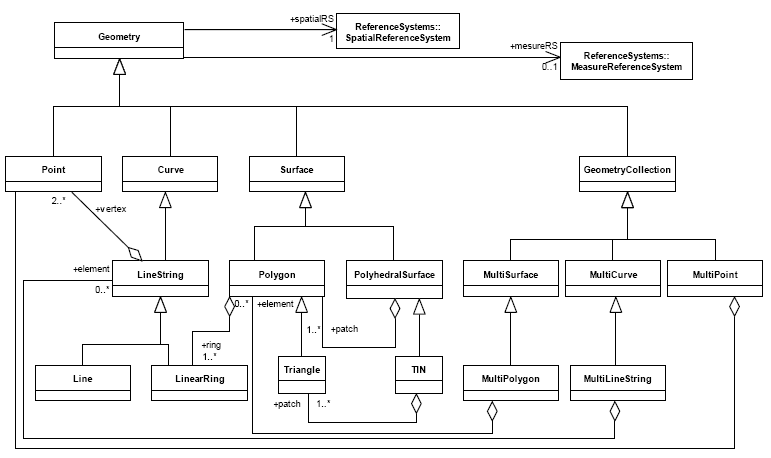
\includegraphics[width=1.2\linewidth]{Immagini/UMLGIS}
	\caption{Diagramma UML di OCS SF}
\end{figure}
Analizziamo ora alcuni tipi degni di nota.

\subsubsection{Point}
Tipo di dato che contiene delle coordinate e dei metodi per accedere a esse.

\subsubsection{Curve}
Oggetto geometrico che estende \texttt{LineString}, è sostanzialmente una sequenza di punti. Gli estremi di questa curva sono chiamati \textbf{frontiera}. Esistono vari tipi di curva:
\begin{itemize}
\item  \textbf{Curva Semplice}: Tipo di curva che non si interseca.
\item \textbf{Curva Chiusa}: Tipo di curva in cui gli estremi coincidono, quindi la frontiera è nulla.
\item \textbf{Anello:} curva semplice e chiusa.
\end{itemize}

\subsubsection{Polygon}
Oggetto geometrico a due dimensioni. Definito da una frontiera esterna e una o più frontiere interne rappresentate da curve chiuse. Una frontiera interna delimita un \textbf{buco}. Le frontiere sono anelli e non si possono intersecare. Un anello può toccare un altro anello solo in un punto tangente. I poligoni devono essere \textbf{validi}, ovvero non devono presentare anomalie.

\begin{figure}[H]
	\centering
	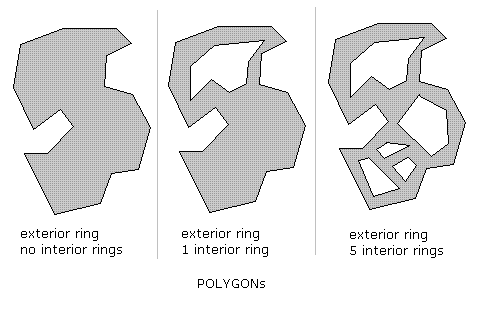
\includegraphics[width=0.5\linewidth]{Immagini/PoliVal}
	\caption{Esempio di Poligoni validi}
\end{figure}

\begin{figure}[H]
	\centering
	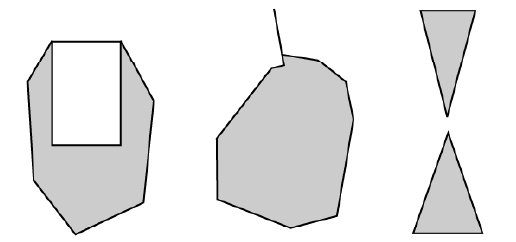
\includegraphics[width=0.5\linewidth]{Immagini/PoliNVal}
	\caption{Esempio di Poligoni non validi}
\end{figure}

Internamente, rappresento un poligono come una sequenza di anelli, ad esempio \texttt{([P1, P2, P3, P4, P1],[P5, P6,P7, P8,P5])}, dove la sequenza più esterna rappresenta la frontiera esterne, mentre le altre sono i buchi.\\
Esiste un tipo \texttt{surface} che estende \texttt{polygon}, che mi permette di calcolare il centro, l'area, capire se un punto è contenuto nel poligono ecc.

\subsection{Geometry Collection}
Collezione di geometrie. Viene esteso da varie classi concrete:
\begin{itemize}
\item \textbf{MultiPoint}: Insieme di \texttt{Point}. Viene detto semplice quando non ci sono due punti uguali.
\item \textbf{MultiLineString}: Insieme di LineString. Fornisce un metodo \texttt{length()} che somma tutte le lunghezze, e un metodo \texttt{isClosed()} che ritorna \texttt{true} se tutte le linee sono chiuse.
\item \textbf{MultiPolygon}: Rappresentazione di collezione poligonale. Gli elementi non possono avere punti in comuni se non punti di contatto su confini.
\end{itemize}

\begin{figure}[H]
	\centering
	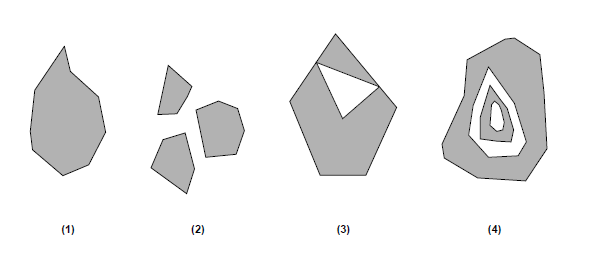
\includegraphics[width=0.5\linewidth]{Immagini/MultiVal}
	\caption{Esempio di MultiPoligono validi}
\end{figure}

\begin{figure}[H]
	\centering
	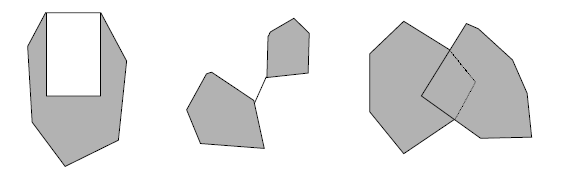
\includegraphics[width=0.5\linewidth]{Immagini/MultiNVal}
	\caption{Esempio di MultiPoligono non validi}
\end{figure}

\subsection{Formati per la rappresentazione geometrica}
Esistono due tipi di formati per la rappresentazione geometrica nelle basi di dati: \textbf{Well-know Text (WKT)} che è un formato testuale, e \textbf{Well-Known Binary (WKB)} che è un formato binario. In una base dati, i dati sono conservati in WKB, ma vengono trasformati in WKT per essere interpretati.

\subsubsection{Esempi di WKT}
Multipunto con 3 punti:\\
\texttt{MULTIPOINT(0 0, 20 20, 60 60)}\\

\noindent Multilinea con 2 linee\\
\texttt{MULTILINESTRING((10 10, 20 20), (15 15, 30 15))}\\

\noindent Multipoligono con 2 poligoni\\
\texttt{MULTIPOLYGON(((0 0,10 0,10 10,0 10,0 0)),((5 5,7 5,7 7,5 7, 5 5)))}\\

\noindent Collezione di geometrie con 2 punti e una linea:\\
\texttt{GEOMETRYCOLLECTION(POINT(10 10), POINT(30 30), LINESTRING(15 15, 20 20))}\\

\subsection{Validità per la rappresentazione Geometrica}
Le geometrie sono \textbf{valide} quando sono costruite correttamente in conformità con lo standard:
\begin{itemize}
\item Geometrie di tipo punto, singole o multiple, sono sempre valide
\item Geometrie di tipo linea, singole o multiple, sono sempre valide purchè la geometria comprenda almeno 2 punti distinti
\item Una geometria singola di tipo poligono è valida se: 
	\begin{itemize}
	\item Ogni è una linea valida con almeno 3 vertici che formano un poligono.
	\item L’anello esterno contiene ogni anello interno
	\item Nessun anello puo’ intersecare se stesso o un altro anello. Un anello tuttavia puo’ avere un numero finito di punti in comune con un altro anello
	\end{itemize}
\item Una geometria multipla di tipo poligono è valida se le singole geometrie sono disgiunte o hanno un numero finito di punti di contatto
\end{itemize}


Posso vedere se sono valide con \texttt{ST\_isValid(Geometry)} appartenente alla classe Geometry. Alcuni sistemi hanno funzionalità aggiunte di validità ad esempio punti duplicati e linee non connesse.

\lessonDate{4 Novembre}
\section{Relazioni e Predicati Spaziali}
Esistono vari tipi di relazioni:
\begin{itemize}
\item \textbf{Relazioni Metriche}: tengono conto della distanza
\item \textbf{Relazioni Topologiche}: tengono conto della forma e della posizione degli oggetti
\item \textbf{Relazioni di Direzioni}: non me ne frega niente
\end{itemize}

\subsection{Relazioni Metriche}
Si basano sul concetto di \textbf{distanza}. Esistono vari concetti di distanza, come la \textbf{distanza di Manhattan}, o il camino minimo in un grafo.\\
La distanza può essere 0 solo se due oggetti \texttt{x} e \texttt{y} sono uguali. Quindi, la distanza fra poligoni non è una distanza accettabile.\\
Nei sistemi di dati spaziali, usiamo due distanze:
\begin{itemize}
\item Distanza euclidea
\item Distanza Geodetica
\end{itemize}

\subsection{Relazioni Topografiche}
Le proprietà topologiche sono caratteristiche che rimangono invarianti anche a seguito di deformazioni (senza strappi).
\begin{figure}[H]
	\centering
	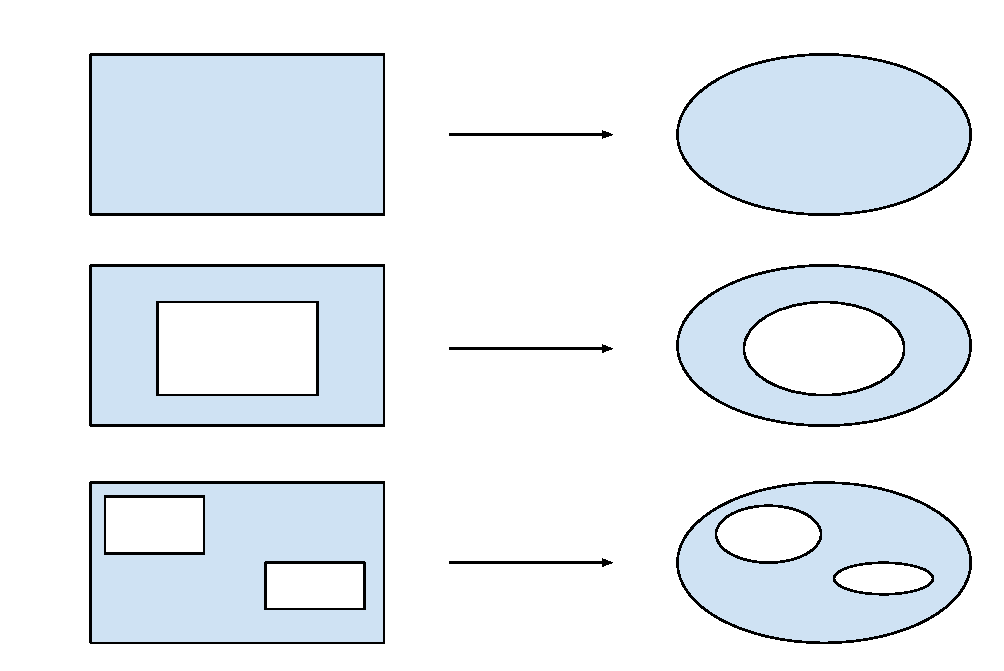
\includegraphics[width=0.5\linewidth]{Immagini/poliTopo}
	\caption{Esempi di poligoni topograficamente equivalenti}
\end{figure}
Ad esempio un quadrato e un'ellisse sono topologicamente equivalenti, perchè posso "stendere" il quadrato in un'ellisse. Ma se metto un buco nello stesso quadrato, non è più equivalente, perchè non posso più riempire il buco.

Considerando una regione topografica, abbiamo:
\begin{itemize}
\item \textbf{Interno} della regione
\item \textbf{Frontiera} insieme di punti del perimetro di una regione
\end{itemize}

Dati due insiemi di punti , il fatto che un'intersezione sia vuota o non vuota è una proprietà topologica. Posso descrivere la relazione topologica fra due oggetti A e B andando a ragionare sui vari rapporti fra frontiere e interni.
\begin{figure}[H]
	\centering
	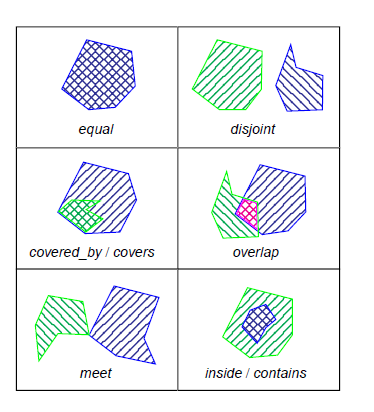
\includegraphics[width=0.5\linewidth]{Immagini/front}
	\caption{Relazioni in rapporto alle frontiere}
\end{figure}
Uso quindi la matrice ottenuta per definire le varie relazioni.
Otteniamo quindi 6 relazioni:
\begin{itemize}
\item equal
\item disjoint
\texttt covered\_by/covers
\item overlap
\item meet
\item inside/contains
\end{itemize}
Se però voglio considerare anche i poligoni con buchi, uso il modello 9 intersection, chiamato così perchè prodotto con una matrice 3x3.\\
Nella formulazione delle varie entità, il punto \textbf{non ha una frontiera}.\\
Con la matrice sopraindicata, ho 512 combinazioni possibili, delle quali me ne interessano solo \textbf{56 significative} nel modello \texttt{DE-9I}.

In questo modello, i valori delle celle sono:
\begin{itemize}
\item \textbf{T}: intersezione non vuota
\item \textbf{F}: intersezione vuota
\item \textbf{*}: valore non rilevante
\item \textbf{0}: dimensione 0
\item \textbf{1}: dimensione 1
\item \textbf{2}: dimensione 2
\end{itemize}
\begin{figure}[H]
	\centering
	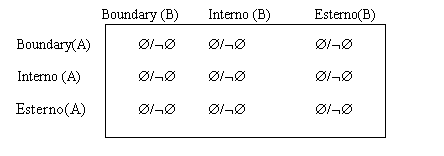
\includegraphics[width=0.8\linewidth]{Immagini/treTreMat}
	\caption{Matrice dei bordi}
\end{figure}
Posso poi convertirle in stringa e usarle in sql. Esistono inoltre una serie di predicati utili a effettuare verifiche su relazioni. \E possibile con l'operatore \texttt{Relate(A,B,string)}, nel quale è possibile inserire un pattern custom.
\begin{itemize}
\item \texttt{Disjoint(A,B)}: torna true se l'intersezione di A e B è vuota
\item \texttt{Intersect(A,B)}: negazione del disjoint
\item \texttt{Touches(A,B)}: Due oggetti si toccano in uno o più punti ma non all'interno
\item \texttt{Crosses(A,B)}: Gli interni di due oggetti si intersecano, ma gli oggetti non sono contenuti l'un l'altro
\item \texttt{Within(A,B)}: A è contenuto in B
\item \texttt{Contains(A,B)}: A contiene B
\item \texttt{Overlaps(A,B)}: Come intersect, ma solo fra oggetti con la stessa dimensione geometrica (aree con aree, linee con linee ecc). L'intersezione deve avere la stessa dimensione geometrica degli elementi comparati. 
\item \texttt{Equals(A,B)}: Quando due geometrie sono uguali, ovvero identificano lo stesso insieme di punti.
\item \texttt{Relate(A,B,string)}: Lo uso per effettuare confronti con relazioni custom
\end{itemize}

Se effettuo dei join utilizzando come condizione dei dati spaziali, parlo di \textbf{join spaziale}.




%\definition{Legge di Brooks}{Aggiungere personale ad un progetto in ritardo lo farà solo ritardare.}

\end{document}v 